\section{Zielsetzung}
\label{sec:Zielsetzung}
Ziel dieses Versuches ist die Absorbitionskoeffizienten von Kupfer und Blei zu bestimmen, indem sie mit $\gamma$-Strahlen beschossen werden.

Für die $\beta$-Strahlung soll ebenfalls die Absorptionskurve aufgenommen werden. Daraus soll die Maximalenergie des $\beta$-Strahlers berechnet werden.

\section{Theorie}
\label{sec:Theorie}
Wenn $\beta$- und $\gamma$- Strahlung auf Materie trifft, treten Wechselwirkungen mit der Materie auf.
Die Häufigkeit der Wechselwirkungen kann dargestellt werden mit dem Wirkungsquerschnitt $\sigma$.
Je größer $\sigma$, desto größer ist die Anzahl der Wechselwirkungen.
Für die $\gamma$ -Strahlung gilt
\begin{equation}
    N(D) = N_0 \text{e}^{-\mu D},
    \label{eqn:Absorptionsgesetz}
\end{equation}
wobei $N(D)$ die Anzahl der Teilchen hinter dem Absorber ist, $N_0$ ist die Ausgangsaktivität, $D$ die Dicke und $\mu$ der Absorbitionskoeffizienten.
Diese Formel wird auch Absorptionsgesetz genannt.
Dieser berechner sich mit
\begin{equation}
    \mu = n \cdot \sigma ,
    \label{eqn:Absorbitionskoeffizienten}
\end{equation}
wobei $n$ die Anzahl der Teilchen innerhalb des Absorbers ist und sich mit
\begin{equation}
    n = \frac{z N_A}{V_{mol}} =\frac{z N_A \rho}{M}
    \label{eqn:AninAb}
\end{equation} 
berechnet. Dabei ist $z$ die Ordnungszahl, $N_A$ die Avogadrokonstante, $V_{mol}$ das Molvolumen, $M$ das Molekulargewicht und $\rho$ die Dichte.

\subsection{Gamma-Strahlung} % (fold)
\label{sub:gamma-Strahlung}
Bei dem Übergang eines Atomkerns von einem höheren Energieniveau zu einem niedrigeren wird die fei werdende Energie in Form eines $\gamma$-Quants abgegeben.
Die emittierten Quanten sind Photonen und breiten sich mit Lichtgeschwindigkeit aus.
Deswegen verhält sich diese Strahlung teilweise wie eine elektromagnetische Welle.
Die Energiezustände die ein Atomkern annehmen kann sind diskret, weswegen es sich bei dem Spektrum eines $\gamma$-Strahlers um ein Linienspektrum handelt.
Die Energie $E$ eines Quants ist gegeben durch $E =h \nu$, wobei $h$ das Planksche Wirkungsquantum ist und $\nu$ die Frequenz des Quants.\\
\subsubsection{Wechselwirkung mit Materie}
\label{subsub:Wechselwirkung}
Für $\gamma$-Energie zwischen $10\si{\kilo\eV}$ und $10\si{\mega\eV}$ treten, abhängig davon womit sie wechselwirken,
verschiedene Effekte auf. Diese werden in \autoref{fig:Abb3} dargestellt.
\begin{figure}[H]
    \centering
    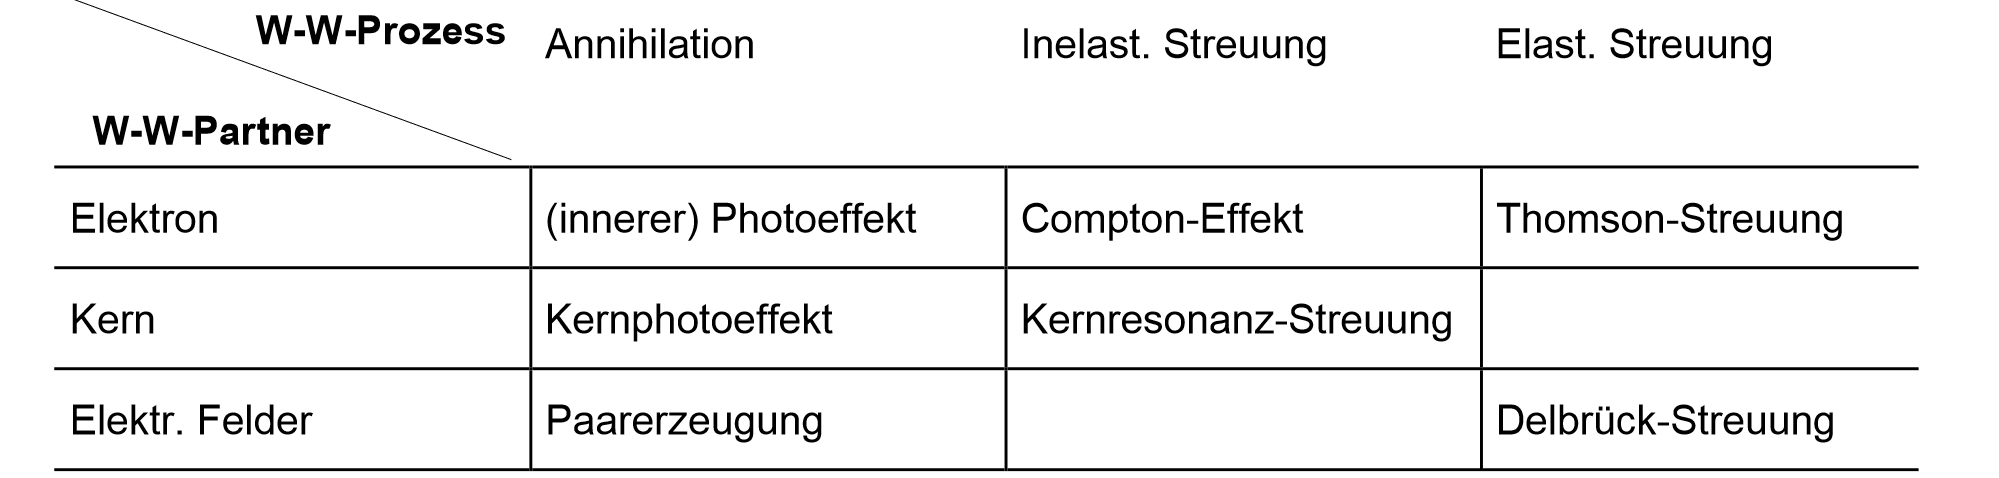
\includegraphics[width=0.7\textwidth]{build/Abb_3.png}
    \caption {Wechselwirkungen von $\gamma$-Strahlung mit Materie\cite[233]{V704}.}
    \label{fig:Abb3}
\end{figure}
In diesem Versuch wird der Photoeffekt, der Compton-Effekt und die Paarbildung betrachtet.\\
Bei dem Photoeffekt wechselwirkt das $\gamma$-Quant mit einem Hüllenelektron, wobei das Elektron aus seiner Schale gelöst wird, wenn die 
$\gamma$-Energie größer ist als die Bindungsenergie des Elektrons.
Die übrigbleibende Energie des Photons wird dann von dem Elektron absorbiert und somit wird das $\gamma$-Quant vernichtet.\\
Der Compton-Effekt ist in \autoref{fig:Abb_4} dargestellt, wobei  ein Quant mit einem freien Elektron wirkt.
Diese Wechselwirkungen ist eine inelastische Streuung und es kommt einer Änderung der Energie und zu einer Richtungsänderung beider Teilchen.
Aus dem Energie- und Impulssatz folgt, dass ein $\gamma$-Quant nie seine ganze Energie auf ein freies Elektron übertragen kann.

\begin{figure}[H]
    \centering
    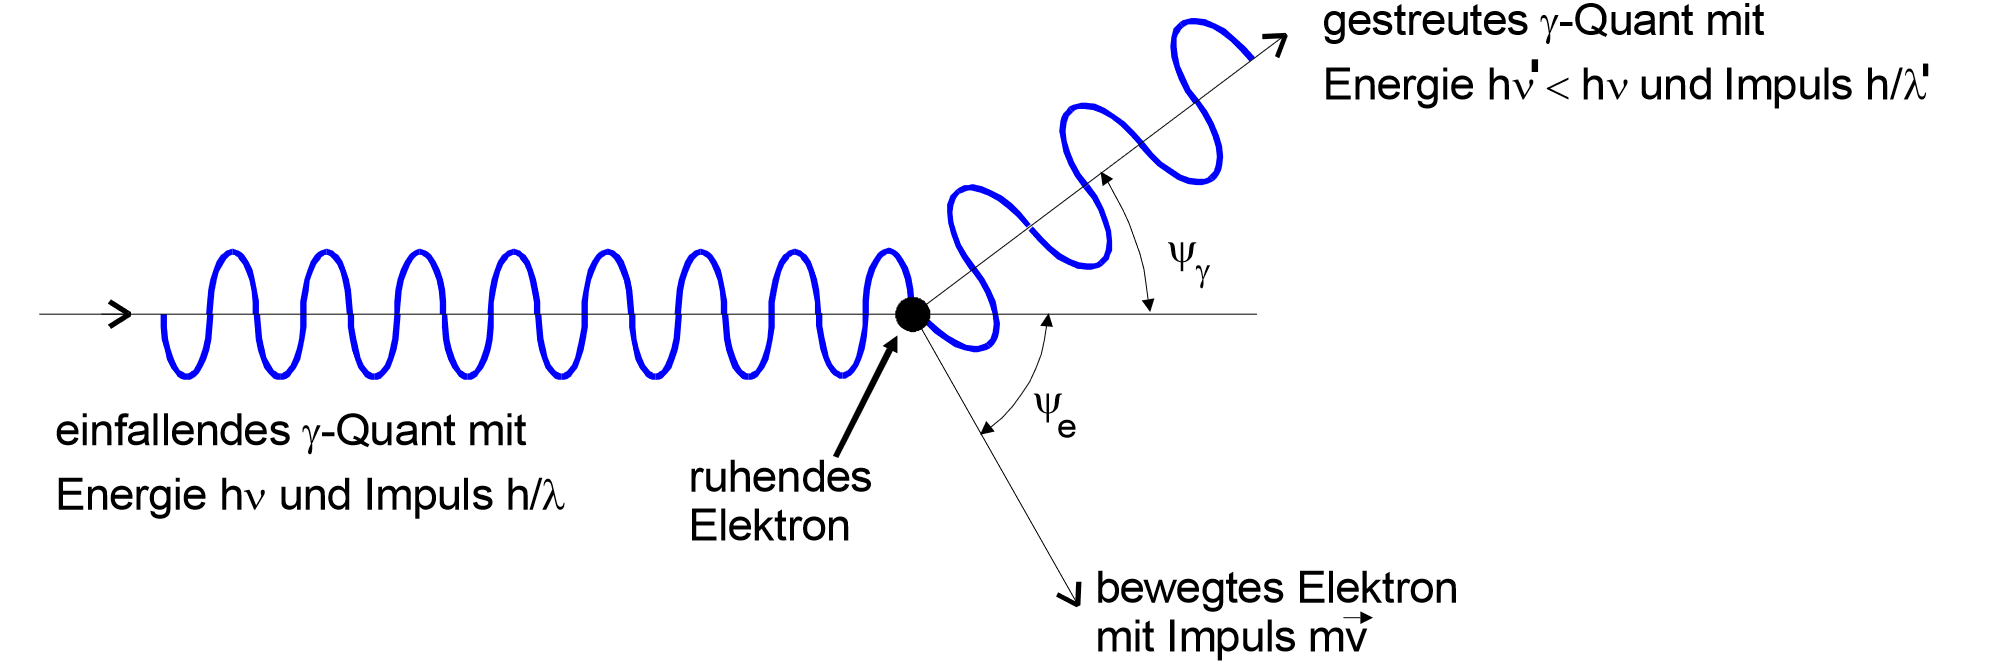
\includegraphics[width=0.5\textwidth]{build/Abb_4.png}
    \caption {Schematische Darstellung des Compton-Streuprozess\cite[234]{V704}.}
    \label{fig:Abb_4}
\end{figure}

Nach dem Streuprozess nimmt die Intensität eines $\gamma$-Strahls aufgrund der Ablenkung ab. 
Der Wirkungsquerschnitt der Compton-Streuung ist durch
\begin{equation}
    \sigma_\mathrm{com}=2\pi\,r_\mathrm{e}^2\left(\frac{1+\epsilon}{\epsilon^2}\left(\frac{2(1+\epsilon)}{1+2\epsilon}-\frac{1}{\epsilon}\ln(1+2\epsilon) \right)+\frac{1}{2\epsilon}\ln(1+2\epsilon)-\frac{1+3\epsilon}{(1+2\epsilon)^2}\right)
    \label{eqn:sigmacom}
\end{equation}
dargestellt. Das Verhältnis der Quantenenergie $E_q$ zur Ruheenergie des Elektrons entspricht $\epsilon = \frac{E_q}{m_0c^2}$ 
und für den Elektronenradius $r_e$ gilt
\begin{equation*}
    r_\mathrm{e}=\frac{e^2}{4\pi\epsilon_0 m_\mathrm{e}c^2}=2,82\cdot10^{-15}\si{\meter},
\end{equation*}
wobei $e_0$ die Elektronenradius ist und $\epsilon_0$ ist die Influenzkonstante.
Der Absorptionskoeffizient kann durch
\begin{equation}
    \mu_\mathrm{com}=\frac{z\,N_\mathrm{A}\,\rho}{M}\sigma_\mathrm{com}
    \label{eqn:Absorptionskoeffizient}
\end{equation}
berechnet werden.\\
Die Paarbildung tritt auf, wenn die Energie des $\gamma$-Quants größer als die doppelte Ruhemasse des Elektrons ist.
Dann wird das $\gamma$-Quant unter der Bildung eines Elektrons und eines Positrons annihiliert.\\
\begin{figure}[H]
    \centering
    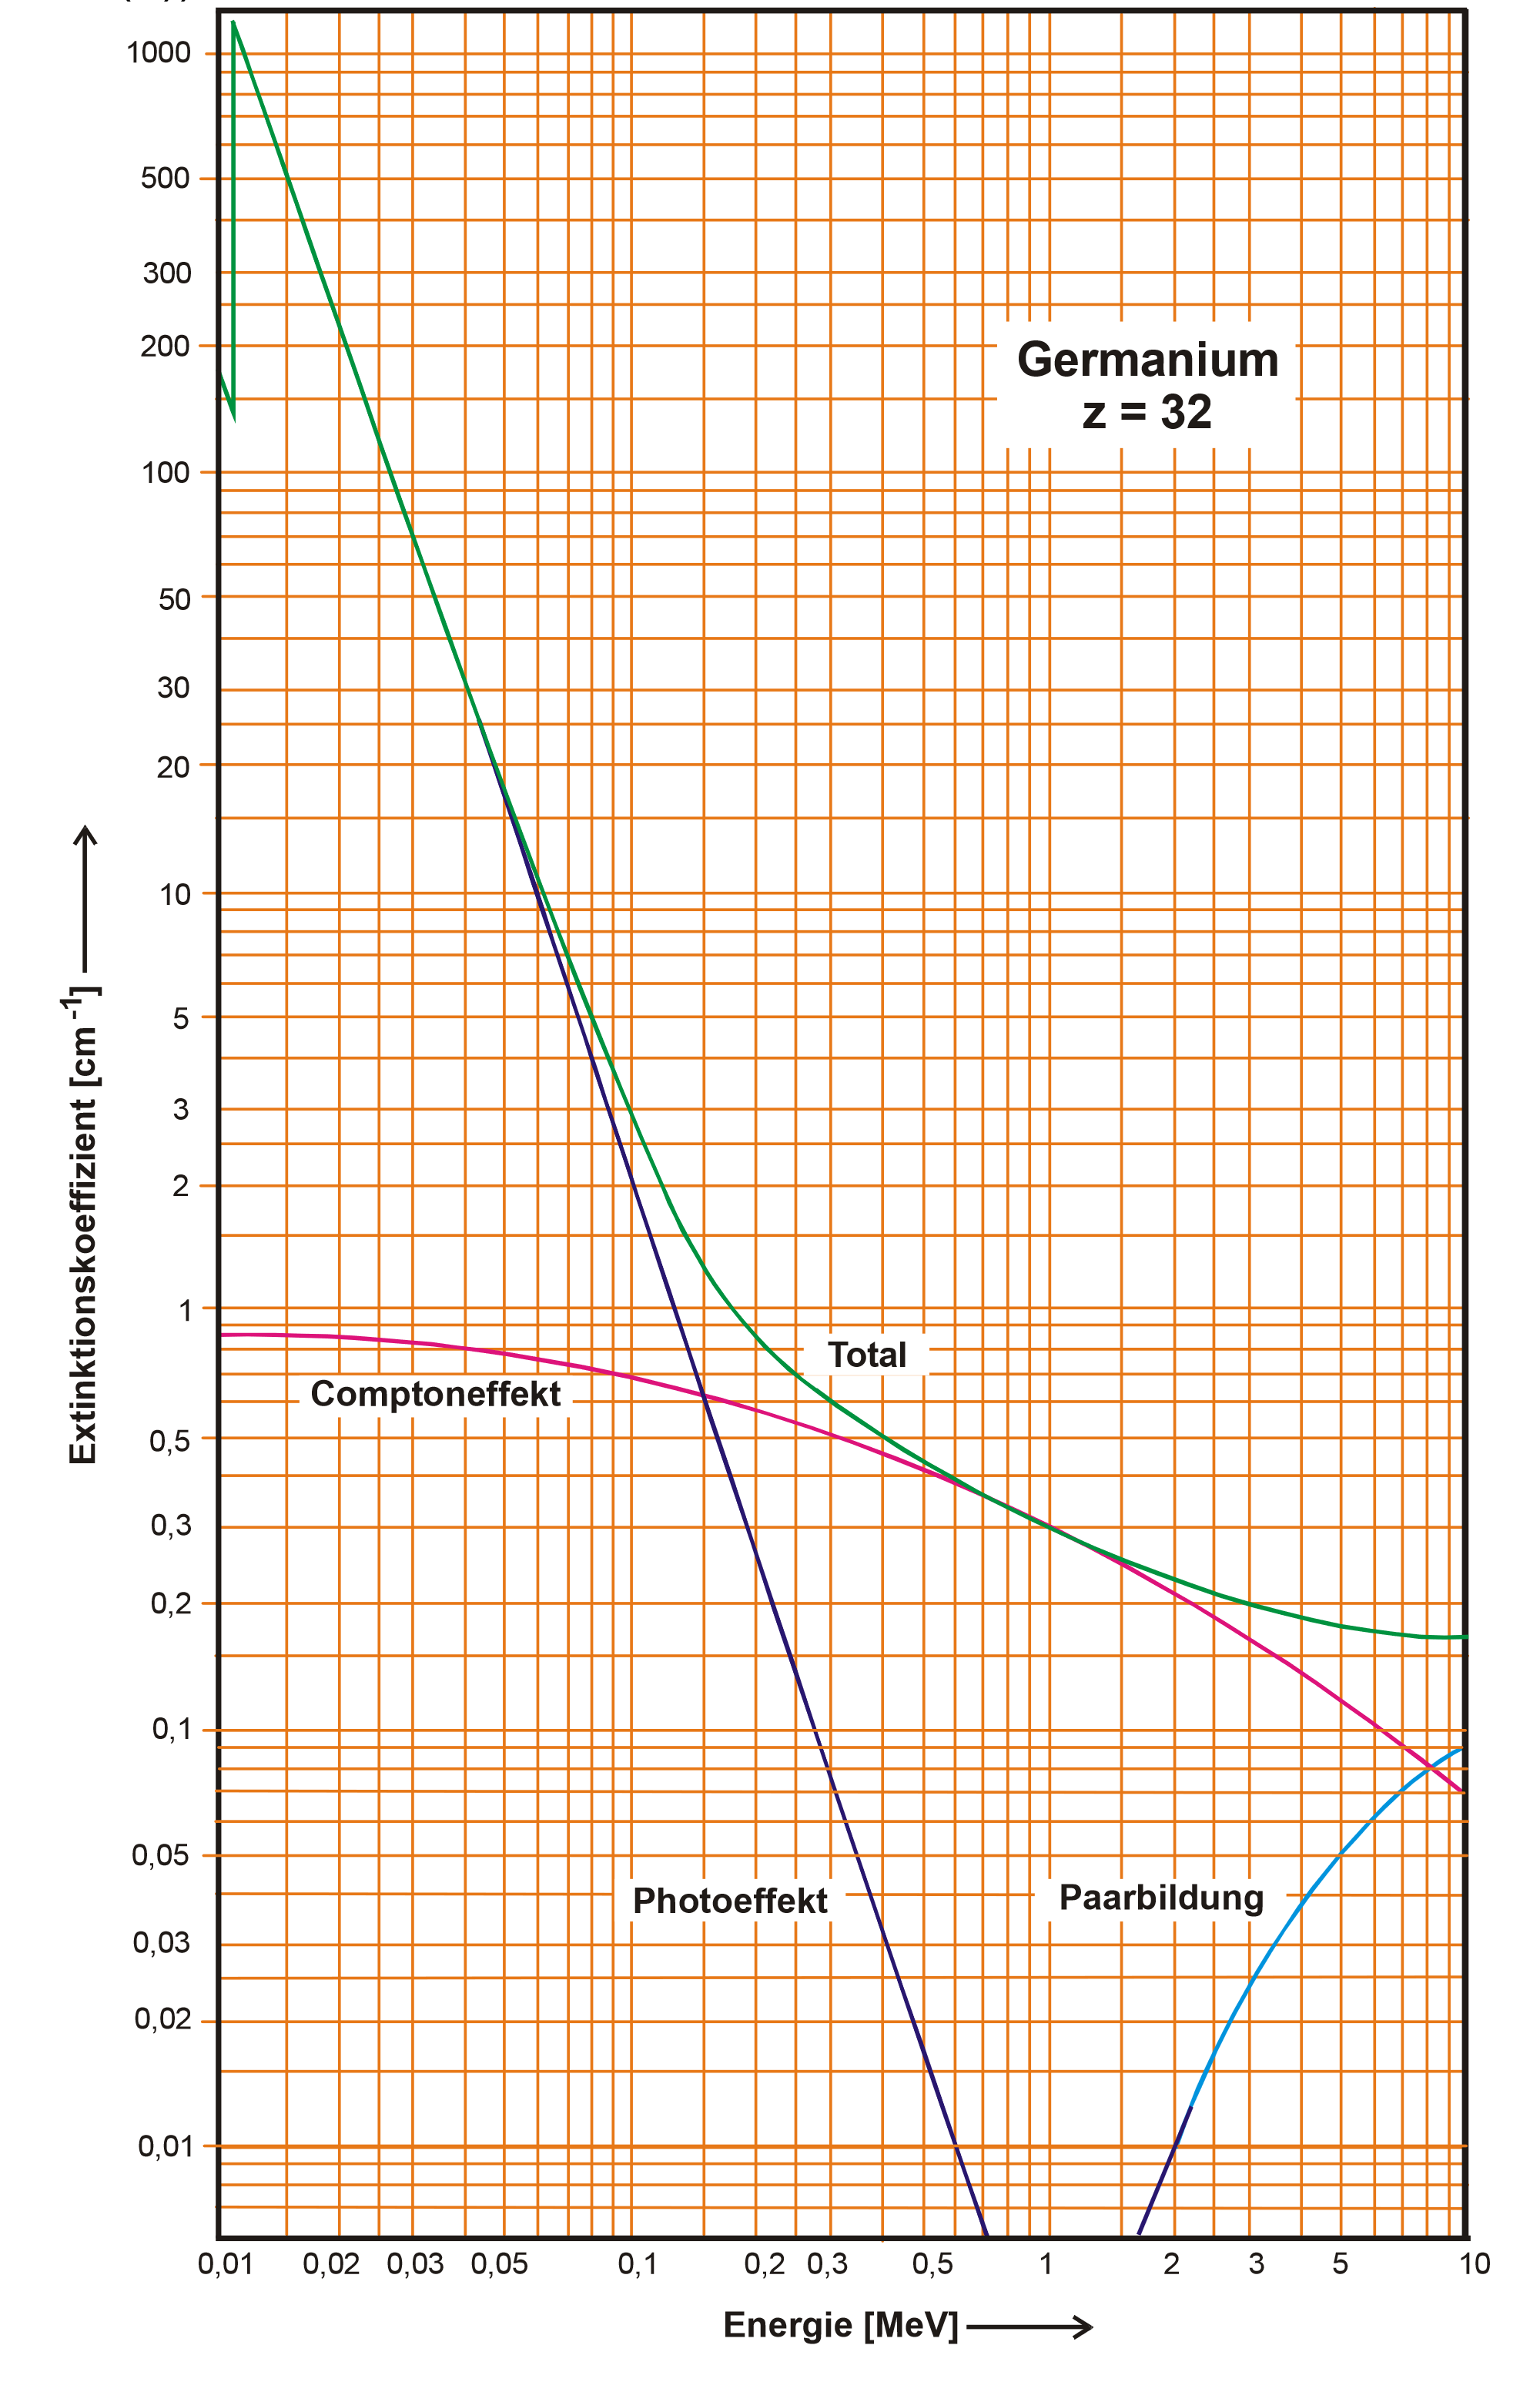
\includegraphics[width=0.5\textwidth]{build/Abb_5.png}
    \caption {Absorptionskoeffizent von Germanium in Abhängigkeit von der Energie\cite[236]{V704}.}
    \label{fig:Abb_5}
\end{figure}
Die drei genannten Effekte treten bei dem Durchgang eines $\gamma$-Strahls durch eine Materieschicht auf, weswegen der Absorptionskoeffizent kompliziert ist.
In \autoref{fig:Abb_5} ist die Energieabhängigkeit des Absorptionskoeffizentfür Germanium dargestellt.
Der Photoeffekt ist dabei für kleine Energien, der Compton-Effekt für mittlere Energien und die Paarbildung für große Energien des $\gamma$-Quants
von entscheidender Bedeutung.
% subsection $\gamma$-Strahlung (end)

\subsection{Beta-Strahlung} % (fold)
\label{sub:Beta-Strahlung}
Bei dem Zerfall von einem Atomkern entsteht $\beta$-Strahlung. Bei dem $\beta^-$-Zefall zerfällt ein Neutron in ein Proton, 
ein Elektron und ein Antineutrino, wobei das Elektron dabei als $\beta$-Teilchen bezeichnet wird.
Der $\beta^+$-Zerfall beschreibt wie ein Proton in ein Neutron, Positron und ein Neutrino zerfällt.
Die Energie verteilt sich dabei beliebig auf die jeweiligen Komponenten, weswegen $\beta$-Strahlung ein kontinuierliches Spektrum.
Die Wechselwirkung des Neutrinos mit der Materie ist so klein, dass sie vernachlässigt werden kann.

\subsubsection{Wechselwirkung mit Materie}
\label{subsub: WeMaB}
Die $\beta$-Teilchen erleiden beim Durchgang durch Materie wesentlich mehr Wechselwirkung als bei $\gamma$-Strahlung.
Im wesentlichen werden hier drei Prozesse voneinander unterschieden.
Es gibt die elastische Streuung am Atomkern des Absorbermaterials, was auch als Rutherford-Streuung bezeichnet wird.
Bei dieser Streuung werden die Elektronen der $\beta$-Strahlung durch die wirkendenden Kräfte des Coulomb-Feld der Atomkerne abgelenkt.
Die Enrgiedifferenz vor und nach der Wechselwirkung ist im Vergleich zu anderen Effekten klein.\\
Eine Wechselwirkung ist die inelastische Streuung, wobei die $\beta$-Teilchen in dem Coulomb-Feld eine Beschleunigung erfahren.
Sie senden gleichzeitig Energie in Form von elektromagnetischet Strahlung ab, wodurch sie wieder abgebremst werden.
Diese wird als Bremsstrahlung bezeichnet.\\
Zuletzt gibt es die inelastische Streuung an einem Elektron.
Dies beschreibt den Prozess der Ionisation und Anregung der Atome des Absorbers. Dabei verlieren die $\beta$-Teilchen nur einen Bruchteil
ihrer Energie. Die Wahrscheinlichkeit dieser Stöße ist proportional zur Anzahl der Elektronen pro Volumenheit und können somit häufig auftreten.
Weswegen durch diesen Prozess $\beta$-Teilchen trotzdem ihre ganze Energie verbrauchen können.\\

\begin{figure}[H]
    \centering
    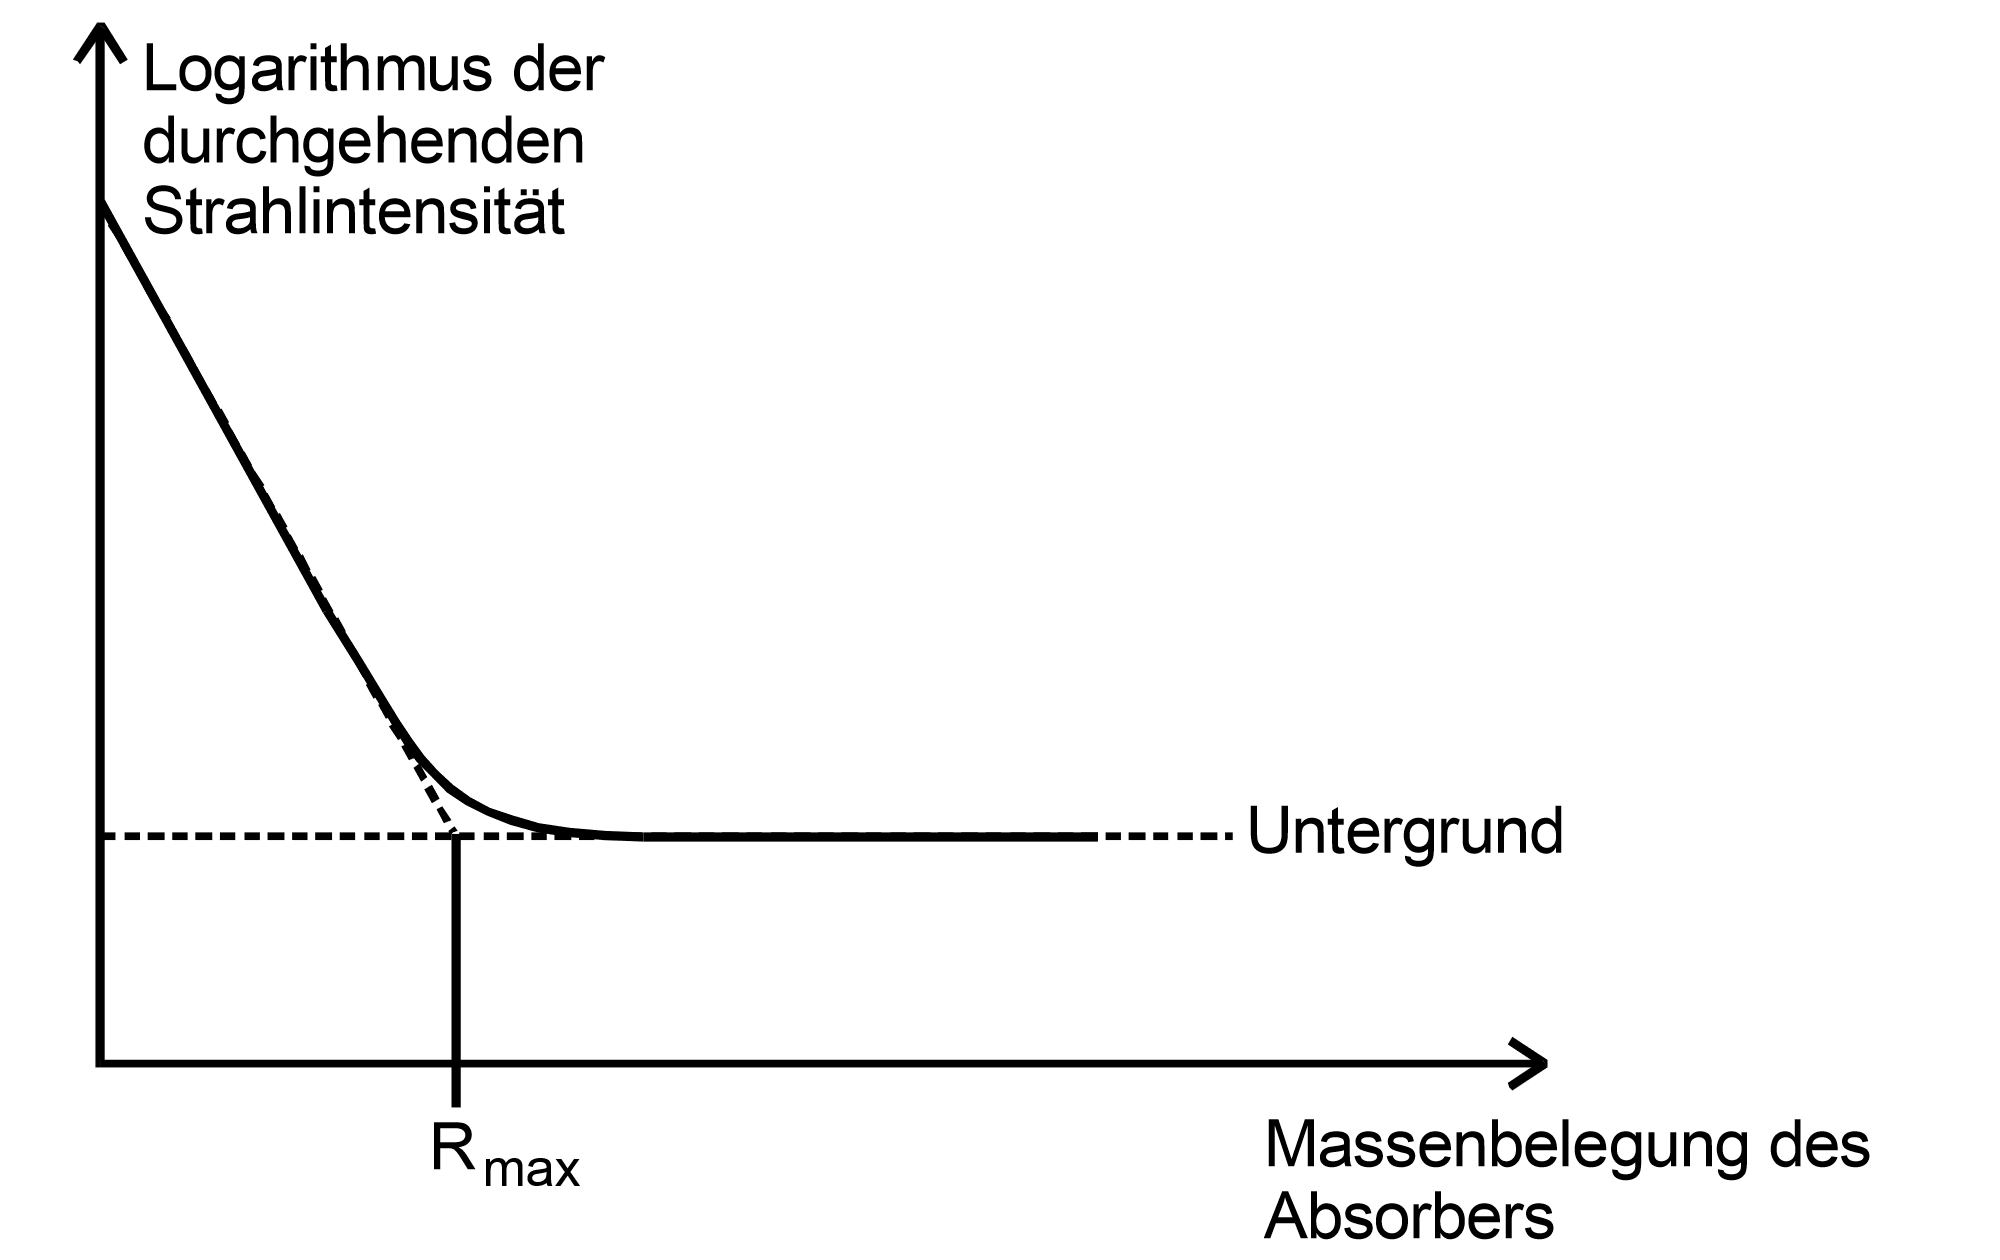
\includegraphics[width=0.5\textwidth]{build/Abb_7.png}
    \caption {Absorptionskurve für einen natürlichen $\beta$-Strahler\cite[241]{V704}.}
    \label{fig:Abb_7}
\end{figure}
Für $\beta$-Teilchen aus natürlicher Quelle gilt bei nicht allzu großen Absorberschichtdicken näherungsweise \autoref{eqn:Absorptionsgesetz}.
Jedoch weicht das Gesetzt bei Schichtdicken in der Nähe der maximalen Massenbelegung $R_{max}$ deutlich ab.
Oberhalb von dieser Reichweite wird dann nur noch die Bremsstrahlung gemessen. Dies wird in \autoref{fig:Abb_7} dargestellt.
$R_max$ ist fast ausschließlich durch die energiereichsten Elektronen bestimmt, weswegen daraus die Größe $E_{max}$ durch
\begin{equation}
    E_{max} = 1,92 \sqrt{R_{max}^2 + 0,22 R_{max}}
    \label{eqn:Emax}
\end{equation}
berachnet werden kann.

% subsection Beta-Strahlung (end)